%===================================== CHAP 2 =================================

\chapter{Theory}

\section{Technical explanation of a Leslie speaker}

\cite{lester_story_leslie_2002}
\cite{Leslie122Manual1971}
\cite{Leslie1949RotatableTremulantSoundProducer}
\cite{TheatreOrgansMysteryLeslie}
\subsection{Explanation of the Effect}

\cite{TheatreOrgansMysteryLeslie} Explains the effect of a Leslie speakers as three main effects happening at once. Because the sound radiated out from the rotating deflector is directional, the intensity of the sound source from a listeneres point will be wariying as the deflector rotates. This effect is called Amplitude Modulation (AM).

sett inn equation.

However \cite{TheatreOrgansMysteryLeslie} as the soundsource is rotating, its relative velocity to the listener will change, causing Frequency Modulation FM as a reslult of the Doppler Effect. As the deflector rotates towards the listener the frequency contnet of the source will be rised and as it rotates away it will be lowered.


%\section{Crossover networks}


\section{Horn Theory}
An acoustic horn is a waveguide that couples a driver to the surrounding air. The primary function of the horn is acoustic impedance transformation: the compression driver at the throat operates into a high acoustic impedance, while free air at the mouth presents a low impedance. By gradually expanding the cross-sectional area, the horn acts as an acoustic transformer, increasing radiation efficiency significantly compared to a bare driver \citep{Kolbrek2008HornTheoryPart1}.

The most common horn profile is the exponential horn (verifiser med kilde), in which the cross-sectional area $S$ increases exponentially along the axis:
\begin{equation}
	S(x) = S_0\,e^{mx}
	\label{eq:horn-area}
\end{equation}
where $S_0$ is the throat area, $x$ is the distance from the throat(noe med acustic centerline), and $m$ is the flare constant that controls the rate of expansion. A key property of the exponential horn is its cutoff frequency \citep{Kolbrek2008HornTheoryPart1}:
\begin{equation}
	f_c = \frac{mc}{4\pi}
	\label{eq:horn-cutoff}
\end{equation}
where $c \approx 343\,\text{m/s}$ is the speed of sound. Below $f_c$ the horn no longer supports propagating waves---acoustic pressure decays exponentially along the axis and radiation is strongly attenuated. Only frequencies above $f_c$ are efficiently radiated, so the choice of flare constant $m$ directly determines the lower bound of the horn's usable frequency range.


\section{Modelling a motor and load with elastic transmission}
The following derivation is based of \citep{egeland2002modeling}.

\begin{figure}[htbp]
	\centering
	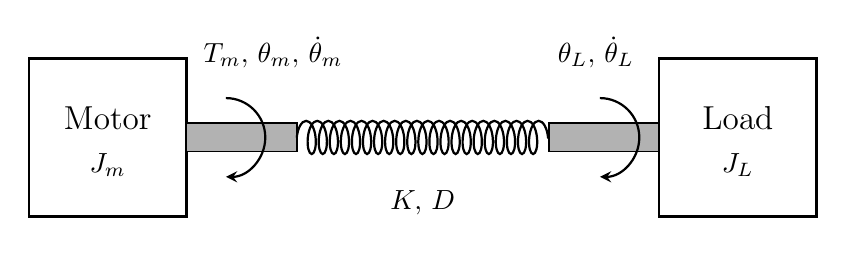
\begin{tikzpicture}[>=stealth, thick]

  % Motor box
  \draw[line width=1pt] (-5,  -1.0) rectangle (-3,  1.0);
  \node at (-4, 0.25) {\large Motor};
  \node at (-4,-0.35) {$J_m$};

  % Motor shaft (left segment)
  \draw[fill=gray!60, draw=black, line width=0.6pt]
    (-3, 0.18) rectangle (-1.6, -0.18);

  % Spring (coil) in the middle
  \draw[decoration={coil, aspect=0.4, segment length=4pt, amplitude=6pt},
        decorate, line width=0.8pt]
    (-1.6, 0) -- (1.6, 0);

  % Load shaft (right segment)
  \draw[fill=gray!60, draw=black, line width=0.6pt]
    (1.6, 0.18) rectangle (3, -0.18);

  % Load box
  \draw[line width=1pt] (3, -1.0) rectangle (5, 1.0);
  \node at (4, 0.25) {\large Load};
  \node at (4,-0.35) {$J_L$};

  % Motor-side labels: T_m, theta_m, omega_m
  \node[above] at (-1.9, 0.75) {$T_m,\,\theta_m,\,\dot{\theta}_m$};

  % Motor-side rotation arrow: half-circle from noon, arrowhead pointing down
  \draw[->, line width=0.8pt]
    (-2.5, 0.5) arc[start angle=90, end angle=-90, radius=0.5];

  % Load-side labels: theta_L, omega_L
  \node[above] at (2.2, 0.75) {$\theta_L,\,\dot{\theta}_L$};

  % Load-side rotation arrow: half-circle from noon, arrowhead pointing down
  \draw[->, line width=0.8pt]
    (2.25, 0.5) arc[start angle=90, end angle=-90, radius=0.5];

  % Spring label K, D
  \node[below] at (0, -0.55) {$K,\,D$};

\end{tikzpicture}

	\caption{Two-mass model of a motor and load connected by an elastic transmission with stiffness $K$ and damping $D$.}
	\label{fig:motor-elastic-load}
\end{figure}

The equations of motion of \autoref{fig:motor-elastic-load} is:
\begin{align}
	J_m \ddot{\theta}_m & = T_m - T_L \label{eq:motor-eom} \\
	J_L \ddot{\theta}_L & = T_L \label{eq:load-eom}
\end{align}

The elstic transmission is modelled as a spring with spring constant K and damper with damping coefficient D resulting in the torque.

\begin{equation}
	T_L = -K\theta_e - D\dot{\theta}_e
	\label{eq:elastic-torque}
\end{equation}

$\theta_e$ is the deflection in the transmission:

\begin{equation}
	\theta_e = \theta_L - \theta_m
	\label{eq:elastic-deflection}
\end{equation}

by introducing the variable $\theta_r$ the derivation becomes more (ett elelr annet).

\begin{equation}
	\theta_r = \theta_m + \frac{J_L}{J_m}\theta_L
	\label{eq:theta-r}
\end{equation}

The equations of motion expressed with $\theta_e$ and $\theta_r$ becomes then

\begin{align}
	\ddot{\theta}_e + \frac{D}{J_e}\dot{\theta}_e + \frac{K}{J_e}\theta_e & = -\frac{1}{J_m}T_m \label{eq:eom-theta-e} \\
	\ddot{\theta}_r                                                       & = \frac{T_m}{J_m} \label{eq:eom-theta-r}
\end{align}

\begin{equation}
	J_e = \frac{J_m J_L}{J}, \quad J = J_m + J_L
	\label{eq:Je}
\end{equation}

The transferfunctions with motor torque as input and angle of the load as output then becomes

\begin{align}
	H_{\theta_m}(s) & : = \frac{\theta_m}{T_m}(s) = \frac{1}{Js^2}
	\frac{1 + 2\zeta_a\frac{s}{\omega_a} + \left(\frac{s}{\omega_a}\right)^2}
	{1 + 2\zeta_1\frac{s}{\omega_1} + \left(\frac{s}{\omega_1}\right)^2}
	\label{eq:Htheta-m}                                            \\[6pt]
	H_{\theta_L}(s) & : = \frac{\theta_L}{T_m}(s) = \frac{1}{Js^2}
	\frac{1 + 2\zeta_1\frac{s}{\omega_1}}
	{1 + 2\zeta_1\frac{s}{\omega_1} + \left(\frac{s}{\omega_1}\right)^2}
	\label{eq:Htheta-L}
\end{align}

\begin{equation}
	\zeta_1 = \frac{D}{2}\frac{1}{\sqrt{J_e K}}, \quad \omega_1 = \sqrt{\frac{K}{J_e}}
	\label{eq:zeta1-omega1}
\end{equation}

\begin{equation}
	\zeta_a = \sqrt{\frac{J_m}{J}}\zeta_1, \quad \omega_a = \sqrt{\frac{J_m}{J}}\,\omega_1 < \omega_1
	\label{eq:zeta-a-omega-a}
\end{equation}


\section{Modelling friction belt drive}
The derivation of the equations of motion in this section is based on section 4.6.5, Belt Drives in \cite{isermann2005mechatronic}. Note that there is a change in the notation.

The belt drive of a typical Leslie speaker is a friction belt drive.
Friction belt drives follow the laws of rope friction. Different examples of friction belt drives include flat belt, round belt and V-belt transmission (TODO: find source confirming V-belt is also a friction belt drive). When correctly designed, these power transmission systems deliver low slip and an almost constant transmission ratio. (TODO: finne kilde om mekanisk støy og legge inn motsetning mot synkronbelte)

In order to develop the equations of motion for the friction belt a set of simplifying assumptions about the system are made:
\begin{itemize}
	\item The belt has no mass.
	\item The distance between the pulley centres are constant.
	\item Centrifugal forces are neglected.
	\item Deformation of pulleys and shafts are negligible compared to belt deformation.
	\item For a certain load, the elasticity of the belt is assumed to follow Hooke's law.
	\item Extension slip only occurs.
\end{itemize}

forklar extension slip (også kalt creep).

The system can be represented with \autoref{fig:belt_drive}.

\begin{figure}[htbp]
	\centering
	% Two-disc belt drive system with parallel spring-damper elements
% Inspired by tikz.net/dynamics_pulley style (Izaak Neutelings)


\begin{tikzpicture}[font=\small]

	%% ──────────────────────────────────────────────────────────────
	%%  GEOMETRY
	%%  Left  disc centre : (0 , 0),  radius r1 = 1.0
	%%  Right disc centre : (9 , 0),  radius r2 = 1.5
	%%  Top  belt tangent : (0, 1.0)  → (9, 1.5),  slope = 0.5/9 ≈ 3.18°
	%%  Bot  belt tangent : (0,-1.0)  → (9,-1.5)
	%%  Perpendicular offset 0.38 → Δy ≈ 0.379 (vertical component)
	%%  At x=2.5: belt y=±1.14  spring y=±1.52  damper y=±0.76
	%%  At x=6.5: belt y=±1.36  spring y=±1.74  damper y=±0.98
	%% ──────────────────────────────────────────────────────────────

	%% ═══════════════════════════════════════════════════════════════
	%%  LEFT DISC
	%% ═══════════════════════════════════════════════════════════════
	\draw[disc] (0,0) circle (1.0);

	% Inertia label
	\node[scale=0.88] at ( 0.00,-0.50) {$J_m$};

	% Centre point + radius label
	\filldraw (0,0) circle (0.07);
	\node[scale=0.85, above right=-2pt] at (0.12,0.08) {$r_m$};

	% Angular-velocity arc (left side, tip pointing downward)
	\draw[force] (110:1.30) arc (110:250:1.30);
	\node[left, scale=0.88] at (-1.30, 0.28) {$\theta_m(t)$};
	\node[left, scale=0.88] at (-1.30,-0.28) {$\dot{\theta}_m(t)$};


	%% ═══════════════════════════════════════════════════════════════
	%%  RIGHT DISC
	%% ═══════════════════════════════════════════════════════════════
	\draw[disc] (9,0) circle (1.5);

	% Inertia label
	\node[scale=0.88] at (9.05,-0.40) {$J_L$};

	% Centre point + radius label
	\filldraw (9,0) circle (0.07);
	\node[scale=0.85, above right=-2pt] at (9.12,0.08) {$r_L$};

	% Angular-velocity arc (right side)
	\draw[force] (9,0) + (-70:1.95) arc (-70:70:1.95);
	\node[right, scale=0.88] at (10.95, 0.30) {$\theta_L(t)$};
	\node[right, scale=0.88] at (10.95,-0.30) {$\dot{\theta}_L(t)$};


	%% ═══════════════════════════════════════════════════════════════
	%%  TOP BELT  — tangent: (0,1.0)→(9,1.5),  slope=0.5/9 ≈ 3.18°
	%%  Spring c_R: (2.5,1.52)→(6.5,1.74)  [+0.379 above belt centre]
	%%  Damper d_R: (2.5,0.76)→(6.5,0.98)  [−0.379 below belt centre]
	%% ═══════════════════════════════════════════════════════════════

	% Outer belt segments along the tangent line
	\draw[belt] (0,1.0) -- (2.5,1.14);
	\draw[belt] (6.5,1.36) -- (9,1.5);

	% Vertical splits at block boundaries
	\draw[belt] (2.5,1.14) -- (2.5,1.52);
	\draw[belt] (2.5,1.14) -- (2.5,0.76);
	\draw[belt] (6.5,1.36) -- (6.5,1.74);
	\draw[belt] (6.5,1.36) -- (6.5,0.98);

	% Spring (top branch) — tilted along belt direction, fewer zigzags
	\draw[spring, decoration={zigzag, amplitude=4pt, segment length=14pt,
			pre length=5pt, post length=5pt}] (2.5,1.52) -- (6.5,1.74);
	\node[above, scale=0.9] at (4.5,1.72) {$c_R$};

	% Damper (bottom branch)
	\draw[damper] (2.5,0.76) -- (6.5,0.98);
	\node[below, scale=0.9] at (4.5,0.50) {$d_R$};

	% Force arrows — LEFT side
	\draw[force] (0.10,1.006) -- (1.00,1.050)
	node[above, midway, scale=0.85] {$F_{tight}$};
	\draw[force] (1.00,1.050) -- (1.90,1.100)
	node[above, midway, scale=0.85] {$F_v$};

	% Force arrows — RIGHT side (pointing leftward toward block)
	\draw[force] (8.90,1.494) -- (7.95,1.441)
	node[above, midway, scale=0.85] {$F_{tight}$};
	\draw[force] (7.95,1.441) -- (7.00,1.388)
	node[above, midway, scale=0.85] {$F_v$};

	% Δl_{tight} displacement arrow (above spring)
	\draw[disp] (3.10,2.24) -- (5.90,2.24);
	\node[above, scale=0.92] at (4.5,2.26) {$\Delta l_{tight}$};


	%% ═══════════════════════════════════════════════════════════════
	%%  BOTTOM BELT  — tangent: (0,-1.0)→(9,-1.5),  slope=−0.5/9
	%%  Damper d_R: (2.5,−0.76)→(6.5,−0.98)  [+0.379 above belt centre]
	%%  Spring c_R: (2.5,−1.52)→(6.5,−1.74)  [−0.379 below belt centre]
	%% ═══════════════════════════════════════════════════════════════

	% Outer belt segments along the tangent line
	\draw[belt] (0,-1.0) -- (2.5,-1.14);
	\draw[belt] (6.5,-1.36) -- (9,-1.5);

	% Vertical splits at block boundaries
	\draw[belt] (2.5,-1.14) -- (2.5,-0.76);
	\draw[belt] (2.5,-1.14) -- (2.5,-1.52);
	\draw[belt] (6.5,-1.36) -- (6.5,-0.98);
	\draw[belt] (6.5,-1.36) -- (6.5,-1.74);

	% Damper (top branch)
	\draw[damper] (2.5,-0.76) -- (6.5,-0.98);
	\node[above, scale=0.9] at (4.5,-0.50) {$d_R$};

	% Spring (bottom branch) — tilted along belt direction, fewer zigzags
	\draw[spring, decoration={zigzag, amplitude=4pt, segment length=14pt,
			pre length=5pt, post length=5pt}] (2.5,-1.52) -- (6.5,-1.74);
	\node[below, scale=0.9] at (4.5,-1.72) {$c_R$};

	% Force arrows — LEFT side
	\draw[force] (0.10,-1.006) -- (1.00,-1.050)
	node[below, midway, scale=0.85] {$F_{slack}$};
	\draw[force] (1.00,-1.050) -- (1.90,-1.100)
	node[below, midway, scale=0.85] {$F_v$};

	% Force arrows — RIGHT side
	\draw[force] (8.90,-1.494) -- (7.95,-1.441)
	node[below, midway, scale=0.85] {$F_{slack}$};
	\draw[force] (7.95,-1.441) -- (7.00,-1.388)
	node[below, midway, scale=0.85] {$F_v$};

	% Δl_{slack} displacement arrow (below spring)
	\draw[disp] (3.10,-2.24) -- (5.90,-2.24);
	\node[below, scale=0.92] at (4.5,-2.26) {$\Delta l_{slack}$};

\end{tikzpicture}

	\caption{Two pulley drive system. Figure recreated from \cite{isermann2005mechatronic}}
	\label{fig:belt_drive}
\end{figure}

The symbols in \autoref{fig:belt_drive} are explained in \autoref{tab:symbol-explaination}.

\begin{table}[h]
	\caption{}\label{tab:symbol-explaination}
	\begin{center}
		\begin{tabular}[c]{l|l}
			\hline
			\multicolumn{1}{c|}{\textbf{Symbol}}    &
			\multicolumn{1}{c}{\textbf{Explanation}}                                                                        \\
			\hline
			$\theta_m(t),\theta_L(t)$               & angular position of motor and load                                    \\
			$\dot{\theta}_m(t),\dot{\theta}_L(t)$   & angular velocity of motor and load                                    \\
			$\ddot{\theta}_m(t),\ddot{\theta}_L(t)$ & angular acceleration of motor and load                                \\
			$J_m, J_L$                              & moment of inertia of motor and load (finn ut om effective eller ikke) \\
			$r_m, r_L$                              & effective radius of motor and load pulley.                            \\
			$F_v$                                   & Pretensioning force.                                                  \\
			$F_{tight}, F_{slack}$                  & force of belt, tight and slack side.                                  \\
			$c_R$                                   & belt spring stiffness factor                                          \\
			$d_R$                                   & belt damping coefficient                                              \\
			$\Delta l_{tight}, \Delta l_{slack} $   & length variation, tight and slack side.                               \\
			\hline
		\end{tabular}
	\end{center}
\end{table}

The spring stiffness factor is assumed to be estimated with
\begin{equation}
	c_R = \frac{EA}{l_R}
	\label{eq:spring_stifness}
\end{equation}
where $EA$ is the spring stiffness factor and $l_R$ is the belt length on the tight or slack side.
(finn ut om hvordan estimere EA)

The belt damping coefficient $d_R$ is given by
\begin{equation}
	d_R = \frac{\Psi c_R}{2\pi\dot{\theta}_{L,0}}
	\label{eq:damping_coeff}
\end{equation}
where $\dot{\theta}_{L,0}$ is the angular velocity of the operating point, and $\Psi$ is the relative damping of the belt which can be experimentally determined (finn ut hvordan).

With these assumptions in place we get the following equation of motion for the motor side using a moment balance
\begin{equation}
	J_m \ddot{\theta}_m(t) = T_m(t) - r_m (F_{tight}(t)-F_{slack}(t))
	\label{eq:motor-side-moment-balance}
\end{equation}
and for the load side
\begin{equation}
	J_L \ddot{\theta}_L(t) = -T_L(t) + r_L (F_{tight}(t)-F_{slack}(t))
	\label{eq:load-side-moment-balance}
\end{equation}

with
\begin{equation}
	F_{tight}(t) = F_v + c_R\Delta l_{tight}(t) + d_R \Delta\dot{l}_{tight}(t)
	\label{eq:tight-force}
\end{equation}

\begin{equation}
	F_{slack}(t) = F_v - c_R\Delta l_{slack}(t) - d_R \Delta\dot{l}_{slack}(t)
	\label{eq:slack-force}
\end{equation}

Inserting \autoref{eq:tight-force} and \autoref{eq:slack-force} into \autoref{eq:motor-side-moment-balance} and \autoref{eq:load-side-moment-balance}, and noting that the pretensioning force $F_v$ cancels, gives:
\begin{equation}
	J_m \ddot{\theta}_m(t) + r_m\bigl[c_R(\Delta l_{tight}(t) + \Delta l_{slack}(t)) + d_R(\Delta\dot{l}_{tight}(t) + \Delta\dot{l}_{slack}(t))\bigr] = T_m(t)
	\label{eq:motor-side-belt-compression}
\end{equation}
and
\begin{equation}
	J_L \ddot{\theta}_L(t) - r_L\bigl[c_R(\Delta l_{tight}(t) + \Delta l_{slack}(t)) + d_R(\Delta\dot{l}_{tight}(t) + \Delta\dot{l}_{slack}(t))\bigr] = -T_L(t)
	\label{eq:load-side-belt-compression}
\end{equation}

Friction belt transmission always operates with a small load-dependent slip. The slip can be described by
\begin{equation}
	s = \frac{v_{m} - v_{L}}{v_m}
	\label{eq:slip-equation}
\end{equation}
where $v_m$ and $v_L$ are the peripheral linear velocities at the motor and load pulleys, given by
\begin{equation}
	v_m = r_m \dot{\theta}_m
	\label{eq:linear-velocity-m}
\end{equation}
\begin{equation}
	v_L = r_L \dot{\theta}_L
	\label{eq:linear-velocity-l}
\end{equation}

Combining \autoref{eq:slip-equation} with \autoref{eq:linear-velocity-m} and \autoref{eq:linear-velocity-l}
gives the actual transmission ratio of the friction belt:
\begin{equation}
	i = \frac{\dot{\theta}_m}{\dot{\theta}_L} = \frac{1}{1-s}\frac{r_L}{r_m} = \frac{i_0}{1-s}
	\label{eq:pulley-ratio}
\end{equation}
where $i_0 = r_L / r_m$ is the ideal (no-slip) transmission ratio.

By applying the extension slip assumption at the break-in and break-out points of both pulleys, and approximating the unknown intermediate belt speeds with the peripheral pulley speeds \cite{isermann2005mechatronic}, the rates of change of the belt length deviations on the tight and slack sides are
\begin{equation}
	\dot{\Delta l}_{tight}(t) = r_m\dot{\theta}_m(t) - \frac{r_L}{1-s}\,\dot{\theta}_L(t)
	\label{eq:dl-tight-rate}
\end{equation}
\begin{equation}
	\dot{\Delta l}_{slack}(t) = (1-s)\,r_m\dot{\theta}_m(t) - r_L\dot{\theta}_L(t)
	\label{eq:dl-slack-rate}
\end{equation}

Using \autoref{eq:pulley-ratio} to substitute $r_L/(1-s) = i\,r_m$, \autoref{eq:dl-tight-rate} and \autoref{eq:dl-slack-rate} become
\begin{equation}
	\dot{\Delta l}_{tight}(t) = r_m\bigl(\dot{\theta}_m(t) - i\,\dot{\theta}_L(t)\bigr)
\end{equation}
\begin{equation}
	\dot{\Delta l}_{slack}(t) = r_m(1-s)\bigl(\dot{\theta}_m(t) - i\,\dot{\theta}_L(t)\bigr)
\end{equation}

Treating $s$ as constant at a given operating point and integrating gives the belt length deviations:
\begin{equation}
	\Delta l_{tight}(t) = r_m\bigl(\theta_m(t) - i\,\theta_L(t)\bigr)
	\label{eq:delta-l-tight}
\end{equation}
\begin{equation}
	\Delta l_{slack}(t) = r_m(1-s)\bigl(\theta_m(t) - i\,\theta_L(t)\bigr)
	\label{eq:delta-l-slack}
\end{equation}

Summing the tight and slack side contributions:
\begin{equation}
	\Delta l_{tight}(t) + \Delta l_{slack}(t) = r_m(2-s)\bigl(\theta_m(t) - i\,\theta_L(t)\bigr)
	\label{eq:delta-l-sum}
\end{equation}
\begin{equation}
	\dot{\Delta l}_{tight}(t) + \dot{\Delta l}_{slack}(t) = r_m(2-s)\bigl(\dot{\theta}_m(t) - i\,\dot{\theta}_L(t)\bigr)
	\label{eq:delta-ldot-sum}
\end{equation}

Substituting \autoref{eq:delta-l-sum} and \autoref{eq:delta-ldot-sum} into \autoref{eq:motor-side-belt-compression} and \autoref{eq:load-side-belt-compression}, and defining the dynamical torsional stiffness $c_{DT}$ and damping coefficient $d_{DT}$ as
\begin{equation}
	c_{DT} = (2-s)\,r_m^2\,c_R \quad \text{[Nm/rad]}
	\label{eq:c-dt}
\end{equation}
\begin{equation}
	d_{DT} = (2-s)\,r_m^2\,d_R \quad \text{[Nm\,s/rad]}
	\label{eq:d-dt}
\end{equation}
one obtains the differential equations of motion for the friction belt drive system:
\begin{equation}
	J_m\ddot{\theta}_m(t) + d_{DT}\bigl(\dot{\theta}_m(t) - i\,\dot{\theta}_L(t)\bigr) + c_{DT}\bigl(\theta_m(t) - i\,\theta_L(t)\bigr) = T_m(t)
	\label{eq:motor-final}
\end{equation}
\begin{equation}
	J_L\ddot{\theta}_L(t) - i_0\bigl[d_{DT}\bigl(\dot{\theta}_m(t) - i\,\dot{\theta}_L(t)\bigr) + c_{DT}\bigl(\theta_m(t) - i\,\theta_L(t)\bigr)\bigr] = -T_L(t)
	\label{eq:load-final}
\end{equation}
Equations \autoref{eq:motor-final} and \autoref{eq:load-final} describe the dynamic behaviour of the friction belt drive as a two-mass oscillator.


\section{Phase-locked Loop}
A phase-locked loop (PLL) is a circuit which has the purpose of synchronizing an output signal
with a reference signal in both phase and frequency \citep[1]{best1993_pll}. In such a case the phase of the output
is said that to locked onto the input signal, therefore giving it its name, phase-locked loop. The first PLLs were introduced in
1932 by the french engineer Henri de Bellescize \cite{deBellescize1932ReceptionSynchrone}, but found its broad indistial application only after becomming available
as an integrated circuit (IC) around 1965 \citep{best1993_pll}. A general PLL can be explained by considering the linear variant,
the linear phase-locked loop (LPLL). Its main operating principles are shown in

\begin{figure}[H]
	\centering
	% PLL block diagram: Phase Detector → Loop Filter → output, VCO feedback
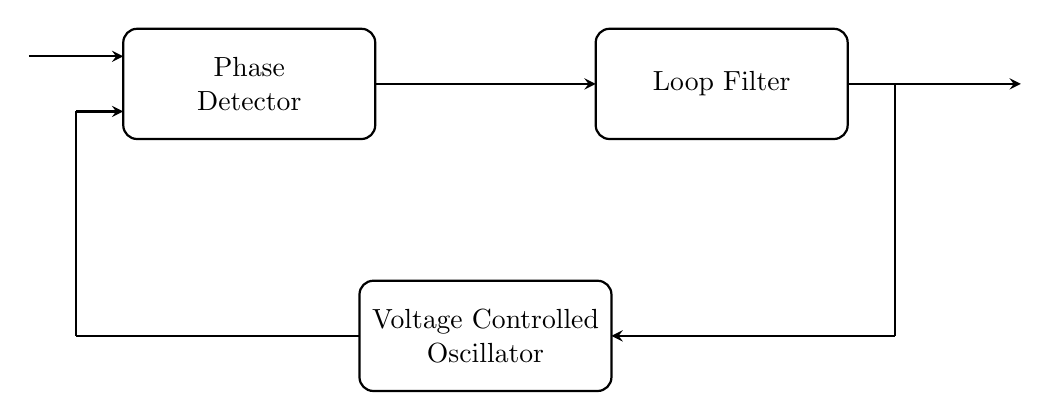
\begin{tikzpicture}[
	box/.style={
		draw, rounded corners=5pt, thick,
		minimum width=3.2cm, minimum height=1.4cm,
		align=center, font=\normalsize
	},
	arr/.style={->, >=stealth, thick},
	line/.style={thick}
]

% Nodes
% PD centre (0,0):  west=(-1.6,0), east=(1.6,0)
% LF centre (6,0):  west=(4.4,0),  east=(7.6,0)
% VCO centre (3,-3.2): west=(1.4,-3.2), east=(4.6,-3.2)
\node[box] (pd)  at (0,   0)    {Phase\\Detector};
\node[box] (lf)  at (6,   0)    {Loop Filter};
\node[box] (vco) at (3,  -3.2)  {Voltage Controlled\\Oscillator};

% Input signal — horizontal arrow into PD, slightly above centre
\draw[arr] (-2.8,  0.35) -- (-1.6,  0.35);

% PD → LF
\draw[arr] (1.6, 0) -- (4.4, 0);

% LF east → junction (0.6 cm outside box) → output arrow
\draw[line] (7.6, 0) -- (8.2, 0);
\draw[arr]  (8.2, 0) -- (9.8, 0);

% Right vertical: junction down to VCO row
\draw[line] (8.2,  0)   -- (8.2, -3.2);

% Arrow from right side into VCO east
\draw[arr]  (8.2, -3.2) -- (4.6, -3.2);

% VCO west → left to left-side vertical
\draw[line] (1.4, -3.2) -- (-2.2, -3.2);

% Left vertical up, then short horizontal arrow into PD, slightly below centre
\draw[line] (-2.2, -3.2) -- (-2.2, -0.35);
\draw[arr]  (-2.2, -0.35) -- (-1.6, -0.35);

\end{tikzpicture}

	\caption{Block diagram of a linear phase-locked loop (LPLL).}
	\label{fig:pll-diagram}
\end{figure}


\subsection{Software Phase-locked Loop}
synchrous communication


\citep{Moore1973PLL} for circuit PLL for motors

\section{Cascade Control}
- fortell om prinsipper for valg av båndbredde mellom loopsene osv

\section{Brushless Direct Current Motor}

The brushless DC (BLDC) motor is known under several different names in the literature. As noted by Hughes \& Drury \citep{hughes2013electric}, the industrial and academic communities have given multiple different names to essentially the same machine, including permanent magnet synchronous motor (PMSM), brushless permanent magnet synchronous motor, brushless AC motor, and permanent magnet servo motor. The term BLDC was originally introduced in the 1970s to describe motors intended as direct replacements for conventional DC motors \cite{hughes2013electric}. While minor differences exist between the variants, they all operate on the same basic principle: a three-phase motor with permanent magnets on the rotor and windings on the stator, where commutation is handled electronically rather than through brushes. (In this thesis, the term BLDC motor is used throughout, as it aligns with the terminology used in the motor datasheet and the moteus c1 controller documentation.)

\subsection{Construction and Governing Effects}
- vis utsnitt av motoren
- forklar de fysiske lovene som genererer dreiemoment.

\subsection{Field Oriented Control}
Introduser med problememene med pwm og sinus control,

%\section{Cogging}
\section{the MIDI Protocol}
MIDI is short for Musical Instrument Digital Interface and is the industry standard for communication between musical equipment \citep{deoliveira2017understandingmidipainlesstutorial}. Instead of communicating the sound signal itself, MIDI transmits messages describing events for instance like which note was played and how intensely it was played, but MIDI can also transmit how knobs were changed which the receiver can interpret to change the sound. Midi has a lot of functionality but only the functionality used in this project will be explained in the following sections.

\subsection{MIDI messages and byte format}
MIDI messages consists consists of a status byte and then optinally up to two databytes. The status byte identifies the message type and which MIDI channel the message is for. The optional data bytes contains the parameters for that message \cite{MMA1996}.
The status bytes and databytes are sepparated by their most significant bit, status bytes using 1 and data byte using 0.
Channel Voice messages are used to send information about a musical preformance on a spesific channel and can command stuff like:
Note On, Note Off, Control Change, Program Change and Pitch Bend. These messages consist of one status byte and two data byte.

System Messages
System Messages are intended for all receivers in the MIDI system. One variant is
System Real Time messages. The Sytem Real Time messages are used to synchronize all clock-based equipment. They consist of only one status byte, and can be one of the following messages:

\begin{itemize}
	\item Timing Clock
	\item Start
	\item Continue
	\item Stop
	\item Active Sensing
	\item System Reset
\end{itemize}
The Real Time messages can be sent at any time and can appear anywhere in the message stream including between a status byte and a system byte of channel voice message.

The timing clock message are used to synchronize, sending the byte F8H 24 times per quarter note.


\subsection{Examples}
\cite{MMA1996}
\cite{deoliveira2017understandingmidipainlesstutorial}


\section{Controller Area Network (CAN)}
\subsection{Message Frame Architecture}
Communication in CAN is done through

\cite{voss2008can}




\subsection{Physical Layer}
\subsection{Bus Arbitration}

\subsubsection{CAN-fd}


\section{Previous Work on this Project}
\label{sec:previous-work}

The work leading into this master's thesis is documented in the project thesis \citep{horpedal2025projectthesis}.
The project started as a hobby project in the spring of 2025.
An IKEA Lunnarp side table was repurposed as an enclosure by cutting a hole for a 12-inch speaker and adding an 8\,mm threaded bar between the base and top plate to support the drum shaft.
The bottom drum was designed in Fusion 360 based on reference pictures of a Leslie speaker drum and laser-cut from 6\,mm MDF, see \autoref{fig:bottom-drum}.

\begin{figure}[H]
	\centering
	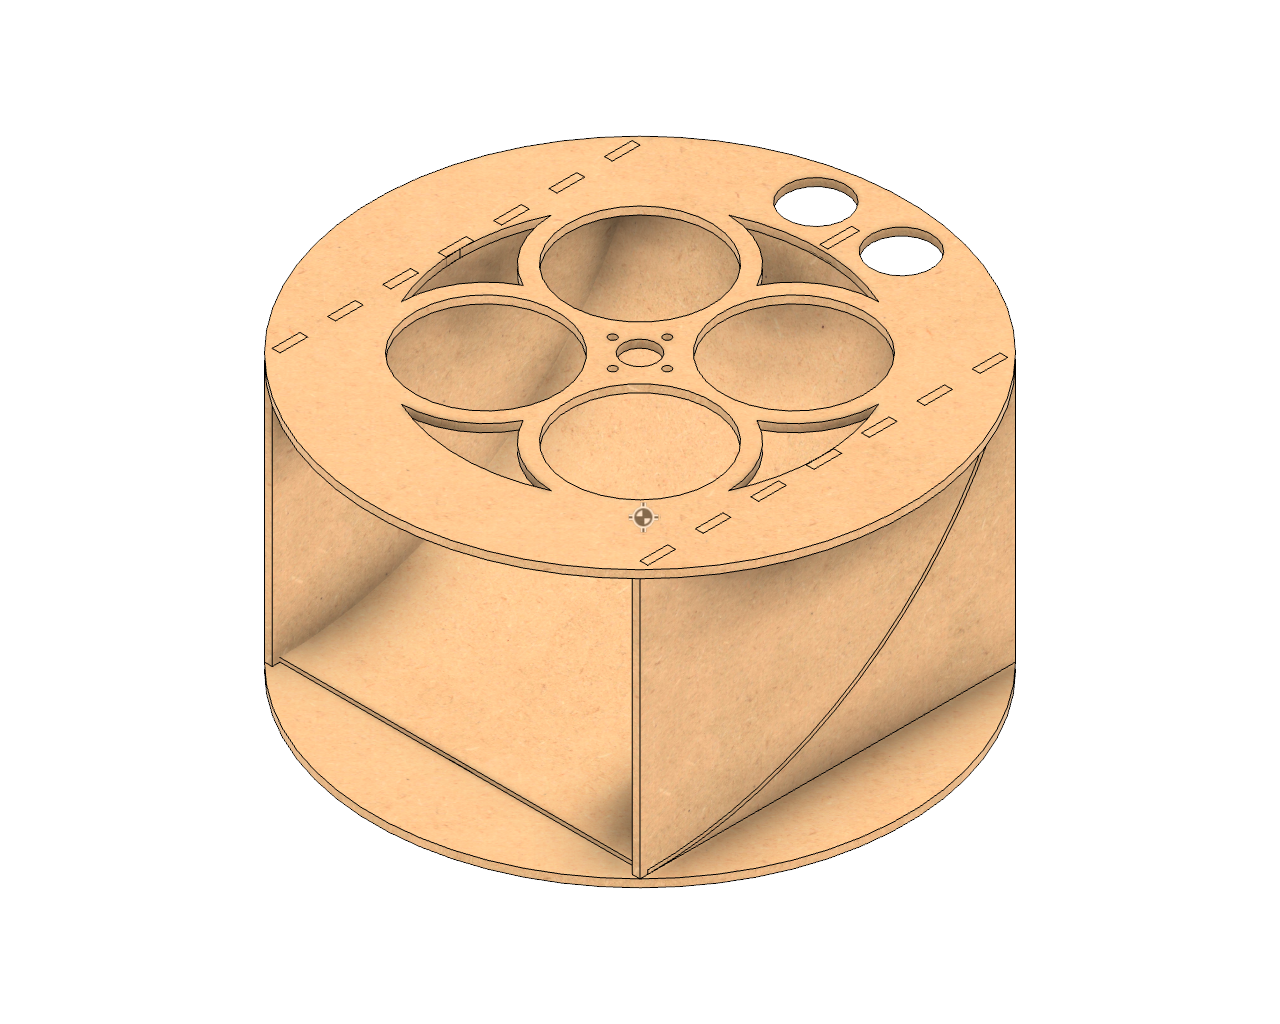
\includegraphics[width=0.45\textwidth]{fig/background/leslie-drum-frontside.png}
	\hfill
	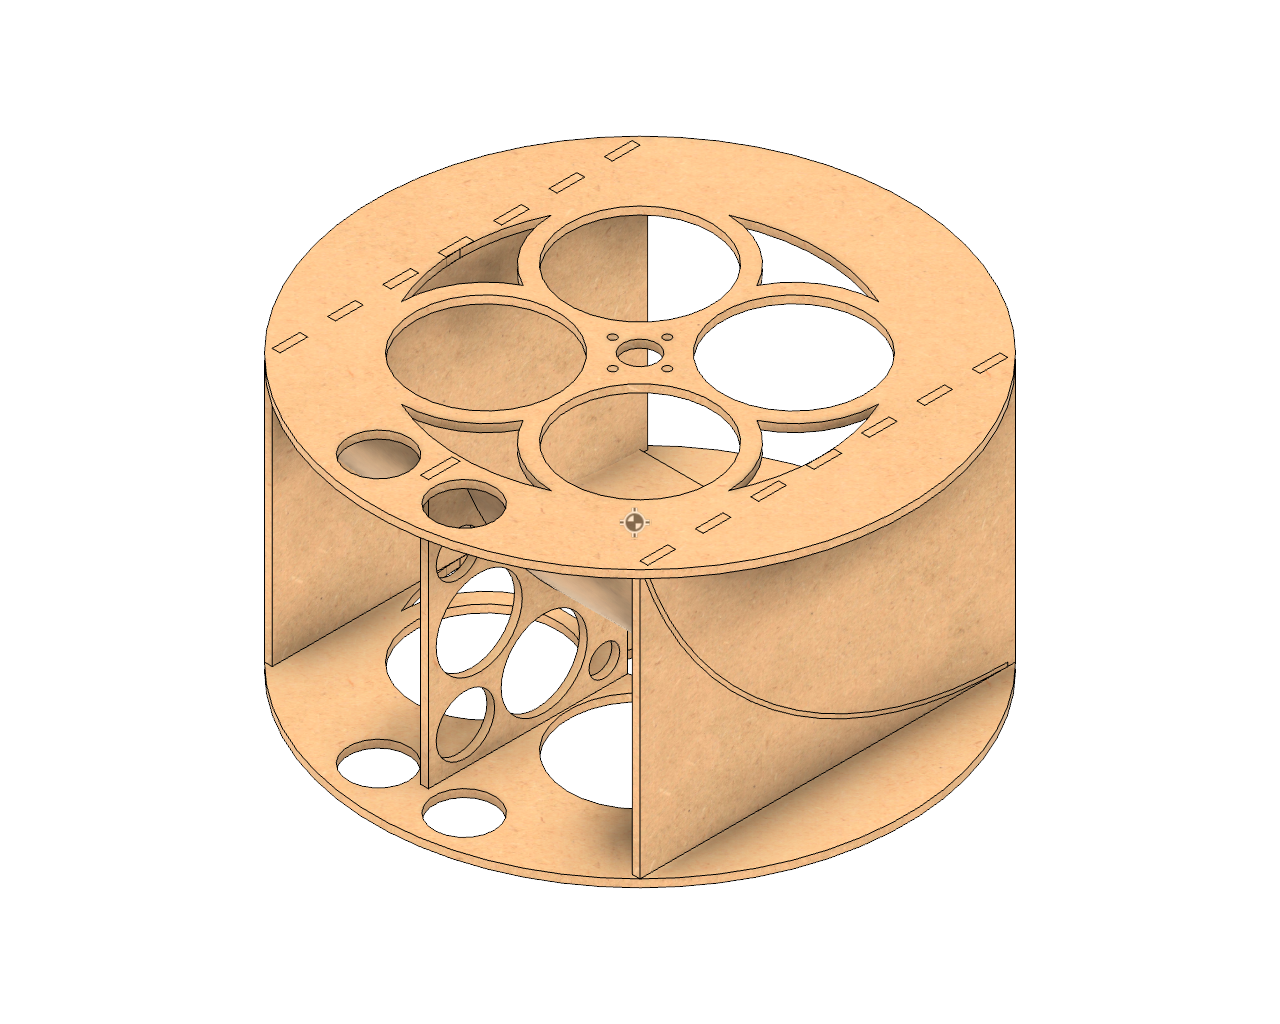
\includegraphics[width=0.45\textwidth]{fig/background/leslie-drum-backside.png}
	\caption{Bottom drum viewed from two different orientations.}
	\label{fig:bottom-drum}
\end{figure}

A BLDC motor (see \autoref{app:motor}), a cheap RioRand motor controller purchased from Amazon with limited documentation, and a 24\,V PSU were sourced and tested.
A polyurethane belt and a 3D-printed PLA drum-side pulley formed a preliminary drive belt system.
A footswitch was also built to allow foot control of the Leslie speed modes.
Its circuit uses charlieplexing to drive three LEDs and read two switches over just three GPIO pins, inspired by \citep{edn_3pins_3leds_3buttons}, see \autoref{fig:footswitch-circuit}, \autoref{tab:charlie-gpio-states}, and \autoref{fig:footswitch-hardware}.

\begin{figure}[H]
	\centering
	\includesvg[width=0.6\textwidth]{fig/background/footswitch-circuit}
	\caption{Footswitch circuit.}
	\label{fig:footswitch-circuit}
\end{figure}

\begin{table}[H]
	\centering
	\small
	\begin{tabular}{lccc}
		\toprule
		Operation     & Pin A      & Pin B      & Pin C      \\
		\midrule
		Light LED A   & HIGH (out) & Hi-Z (in)  & LOW (out)  \\
		Light LED B1  & LOW (out)  & HIGH (out) & Hi-Z (in)  \\
		Light LED B2  & Hi-Z (in)  & LOW (out)  & HIGH (out) \\
		Read switch A & IN+PULLUP  & LOW (out)  & Hi-Z (in)  \\
		Read switch B & Hi-Z (in)  & IN+PULLUP  & LOW (out)  \\
		\bottomrule
	\end{tabular}
	\caption{GPIO configuration of pins A, B, and C for LED driving and switch reading.}
	\label{tab:charlie-gpio-states}
\end{table}

\begin{figure}[H]
	\centering
	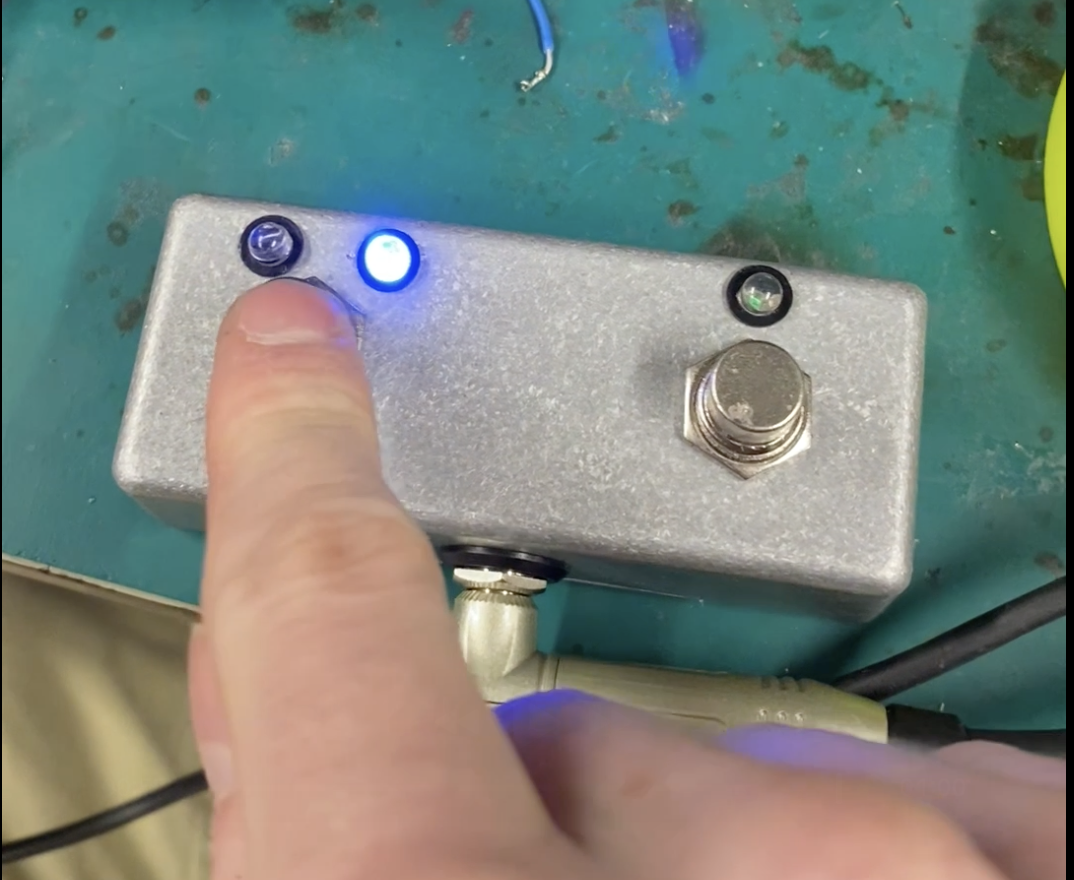
\includegraphics[width=0.6\textwidth]{fig/background/footswitch-hardware.png}
	\caption{Previously implemented footswitch.}
	\label{fig:footswitch-hardware}
\end{figure}

\label{sec:foot}
Building on this foundation, the project thesis extended the system.
A spring-loaded belt tensioner and a 3D-printed motor shaft support were added to improve drive belt stability.
Because the RioRand controller offered no position feedback and belt slip was observed during rapid deceleration, a custom infrared quadrature encoder was designed and mounted directly on the drum to measure angular position and velocity independently of the motor, providing 32 counts per revolution.
An Arduino Nano ESP32 running FreeRTOS served as the main controller, communicating with the Leslie over USB-MIDI.
The software implemented cascaded velocity and position control, discrete (\textsc{Chorale}/\textsc{Stop}/\textsc{Tremolo}) and continuous MIDI modes, trajectory generation with configurable rise and fall times, and a homing procedure to return the drum to a repeatable angle when stopped.
The Leslie effect was demonstrated and audio recordings confirmed it was clearly perceptible, particularly at high rotational speeds.

Several limitations remained at the end of the project thesis.
The RioRand motor controller acted as a black box with unknown internal control laws and no diagnostics, and ultimately failed during the final recording session.
The 32-count encoder resolution (11.25° per count) was too coarse for precise position control and introduced quantization noise in velocity estimation.
Mechanical noise from the belt drive was audible at higher speeds, and no horn assembly existed for high-frequency content.

\cleardoublepage




